\documentclass[12pt, titlepage]{article}

\usepackage{booktabs}
\usepackage{tabularx}
\usepackage{longtable}
\usepackage{hyperref}
\usepackage{xcolor}
\usepackage{graphicx}
\usepackage{float}

\hypersetup{
    colorlinks,
    citecolor=black,
    filecolor=black,
    linkcolor=red,
    urlcolor=blue
}
\usepackage[round]{natbib}

 %% Comments

\usepackage{color}

\newif\ifcomments\commentstrue %displays comments
%\newif\ifcomments\commentsfalse %so that comments do not display

\ifcomments
\newcommand{\authornote}[3]{\textcolor{#1}{[#3 ---#2]}}
\newcommand{\todo}[1]{\textcolor{red}{[TODO: #1]}}
\else
\newcommand{\authornote}[3]{}
\newcommand{\todo}[1]{}
\fi

\newcommand{\wss}[1]{\authornote{blue}{SS}{#1}} 
\newcommand{\plt}[1]{\authornote{magenta}{TPLT}{#1}} %For explanation of the template
\newcommand{\an}[1]{\authornote{cyan}{Author}{#1}}

 %% Common Parts

\newcommand{\progname}{ProgName} % PUT YOUR PROGRAM NAME HERE
\newcommand{\authname}{Team \#, Team Name
\\ Student 1 name and macid
\\ Student 2 name and macid
\\ Student 3 name and macid
\\ Student 4 name and macid} % AUTHOR NAMES                  

\usepackage{hyperref}
    \hypersetup{colorlinks=true, linkcolor=blue, citecolor=blue, filecolor=blue,
                urlcolor=blue, unicode=false}
    \urlstyle{same}
                                


\begin{document}

\title{Verification and Validation Report: \progname} 
\author{\authname}
\date{\today}
	
 \maketitle

\pagenumbering{roman}

\section{Revision History}

\begin{tabularx}{\textwidth}{p{3cm}p{2cm}X}
\toprule {\bf Date} & {\bf Version} & {\bf Notes}\\
\midrule
March 2 & 1.0 & Created base template for report\\
March 2 & 1.1 & Conducted system tests and added their results\\
March 3 & 1.2 & Added unit tests and their traceability\\
March 4 & 1.3 & Added NFR tests and their results \\
March 7 & 1.4 & Added unit test results \\
March 8 & 1.5 & Finished remaining sections of the document \\
\bottomrule
\end{tabularx}

~\newpage

\section{Symbols, Abbreviations and Acronyms}

\renewcommand{\arraystretch}{1.2}
\begin{tabular}{l l} 
  \toprule		
  \textbf{symbol} & \textbf{description}\\
  \midrule 
  T & Test\\
  LaTeX, TeX & A professional document writing software and compiler\\
  GitHub & A version control software hosted by Microsoft\\
  \bottomrule
\end{tabular}\\

%\wss{symbols, abbreviations or acronyms -- you can reference the SRS tables if needed}

\newpage

\tableofcontents

\listoftables %if appropriate

\listoffigures %if appropriate

\newpage

\pagenumbering{arabic}

This document ...

\section{Functional Requirements Evaluation}

\subsection{GitHub}
\begin{center}
    \begin{longtable}{|c|p{1cm}|p{2.7cm}|p{3cm}|p{3cm}|c|}
        \caption{GitHub System Tests \label{long}}\\
        \hline
        \textbf{Id} & \textbf{Req Id} & \textbf{Input} & \textbf{Expected Result} & \textbf{Actual Result} & \textbf{Result}   \\
        \hline
        ST-1 & FR5, FR6, FR7 & The authenticated user creates a project through UnderTree, adds collaborators and provides a valid name for the project & A new project is created and displayed on UnderTree & The user views the new project in their projects list along with the repository in their GitHub & \textcolor{green}{PASS} \\
        \hline
        ST-2 & FR5 & The authenticated user creates a project through UnderTree, adds collaborators and provides a invalid name for the project & An error appears that the name already exists in GitHub & The user encounters an error of invalid project name & \textcolor{green}{PASS} \\
        \hline
        ST-3 & FR8, FR9, FR10 & The authenticated user views a list of their GitHub repositories and chooses the ones to import & The user sees the projects imported onto their projects page & The user is able to view the imported projects & \textcolor{green}{PASS} \\
        \hline
        ST-4 & FR40, FR41 & The authenticated user clicks the git log button to view the list of commit history & The user sees the past 10 commits created on GitHub & The user is able to view the 10 previous commits & \textcolor{green}{PASS} \\
        \hline
        ST-5 & FR45 & The authenticated user selects the files to commit, clicks the git commit button & The user is able to create a commit message & The user is able to create a commit message & \textcolor{green}{PASS} \\
        \hline
        ST-6 & FR46, FR47 & The authenticated user selects the files to commit, clicks the git commit button, enters a commit message and pushes the commit & The user is able to view the changes from UnderTree onto the GitHub & The user is able to push the changes and view them on GitHub with the corresponding users & \textcolor{green}{PASS} \\
        \hline
    \end{longtable}
\end{center}

\subsection{Authentication}
\begin{center}
    \begin{longtable}{|c|p{1cm}|p{2.7cm}|p{3cm}|p{3cm}|c|}
        \caption{Authentication System Tests \label{long}}\\
        \hline
        \textbf{Id} & \textbf{Req Id} & \textbf{Input} & \textbf{Expected Result} & \textbf{Actual Result} & \textbf{Result} \\
        \hline
        ST-7 & FR3 & User is not authenticated and clicks the login button to be redirected to the GitHub & The user is able to log in and a JWT token is stored as a cookie & The user is able to log in and can validate the cookie in the browser & \textcolor{green}{PASS} \\
        \hline
        ST-8 & FR3 & User is not authenticated and clicks the login button to be redirected to the GitHub and enters the wrong credentials & The user is not able to log in & The user is not able to log in & \textcolor{green}{PASS} \\
        \hline
        ST-9 & FR3 & User is already logged in and attempts to log in again & The user is redirected to projects page & The user is redirected to projects page & \textcolor{green}{PASS} \\
        \hline
        % ST-10 & FR4 & User is not authenticated and clicks the login button to be redirected to the GitHub and enters the right credentials & The user is not able to log in and redirected to the projects page & The user is not able to log in and gets redirected to the login page & \textcolor{green}{PASS} \\
        % \hline
        % ST-44 & FR4 & User tries to access a secure route in the system without being authenticated & The user is not able to complete the operation and is redirected to the login page & The user is redirected to login & \textcolor{green}{PASS} \\
        % \hline
        ST-10 & FR4 & User is logged in with an invalid JWT token and tries to complete an operation in the system & The user is redirected to the login page and the JWT token in the cookie is removed & The user is redirected to the login page and can view the missing cookie in the browser & \textcolor{green}{PASS} \\ 
        \hline
        ST-11 & FR4 & User is logged in and clicks the log out button & The user is redirected to the home page and their lack of authentication is reflected in the database & The user is redirected to the home page and the user is not authenticated in the database & \textcolor{green}{PASS} \\
        \hline
        % ST-45 & FR4 & User tries to complete an operation in the system with expired tokens & The user is able to continue with a renewed token & The user completes the operation as desired & \textcolor{green}{PASS} \\
        % \hline
    \end{longtable}
\end{center}

\subsection{Editor}

\begin{center}
    \begin{longtable}{|c|p{1cm}|p{2.7cm}|p{3cm}|p{3cm}|c|}
        \caption{Editor System Tests \label{long}}\\
        \hline
        \textbf{Id} & \textbf{Req Id} & \textbf{Input} & \textbf{Expected Result} & \textbf{Actual Result} & \textbf{Result}\\
        \hline
        ST-12 & FR18, FR19 & User clicks create new file, fills in new file name and click confirm & File is displayed in the file menu and is also added to the list of files in the database &  File is displayed in the file menu and is also added to the list of files in the database &  \textcolor{green}{PASS} \\
        \hline
        ST-13 & FR20 & User moves cursor position & The new cursor position is reflected in the user's and collaborating user's editor & The new cursor position can be seen from the every user's editor &  \textcolor{green}{PASS} \\
        \hline
        ST-14 & FR22 & User types latex specific code in the editor & The latex code should be highlighted accordingly & The latex code is highlighted accordingly &  \textcolor{green}{PASS}  \\
        \hline
        ST-15 & FR23 & User types normal text with some spelling errors into the editor & The words with the spelling error should be highlighted & No highlighting is done  &  \textcolor{red}{FAIL} \\
        \hline
        ST-16 & FR21 & All the different users make an different edit to the same files using the editor & The updated file should have all those changes and should be the same for all the users & All users can see the changes without any issues and the file state is the same for all users  &  \textcolor{green}{PASS} \\
        \hline
        ST-17 & FR29 & User selects the option to delete one of the file from the file list & A confirmation dialog confirming the user to delete the file should
appear &  A modal appears asking the user to confirm &  \textcolor{green}{PASS} \\
        \hline
        ST-18 & FR21, FR30 & One of the user deletes a file that multiple users have open & All of the users should not longer be able to see the file in the editor & The users are only unable to see the file after reloading the page & \textcolor{green}{PASS} \\
        \hline
        ST-19 & FR31, FR32 & User selects the option to rename one of the file from the file list & he user is allowed to enter the new name for the file & A modal appears asking the user to enter a new name for the file & \textcolor{green}{PASS} \\
        \hline
        ST-20 & FR33 & User selects the option to rename one of the file from the file list, and renames it to a different name & This event of the file being renamed should be recorded in the client side storage alongside the user who made the change & The event is stored in the local storage & \textcolor{green}{PASS}  \\
        \hline
        ST-21 & FR21, FR32 & One of the user renames a file that multiple users have open & All of the users should should see the updated file name in the editor & he users are only unable to see the updated file after reloading the page & \textcolor{green}{PASS} \\
        \hline
        ST-22 & FR24, FR25, FR26 & User selects the option to create a new file & he system should present the user with modal that prompts the user for the name and the extension of the file, with default name and .tex extension filled in & The modal presents an empty input field &  \textcolor{red}{FAIL} \\
        \hline
        ST-23 & FR26 & User selects confirm on the new file creation modal & The empty file should be added to the editor, and should also be visible to other users & The new file is displayed in the filemenu &  \textcolor{green}{PASS} \\
        \hline
        ST-24 & FR21, FR26 & Each user creates a new file & ach user should be able to see all the files created by the other users in the editor & The new file created by each member is visible to the others & \textcolor{green}{PASS}  \\
        \hline
        ST-25 & FR27 &  User selects the option to upload a file & he user should be presented a modal to choose their local file & The user is presented with a modal with a file input field that allows the user to select a file from their device &  \textcolor{green}{PASS}  \\
        \hline
        ST-26 & FR28 & User browses through and chooses a local file to upload & he file should appear in the file list window with the same name and extension as the local file chose to upload with the same file content & The selected file is displayed in the filemenu and the content remains the same & \textcolor{green}{PASS} \\
        \hline
        ST-27 & FR34 & User tries to insert, delete and modify the text in the latex file & Each action should be carried out without any issues & Each action is carried out without any issues & \textcolor{green}{PASS} \\
        \hline
        ST-28 & FR35 & User tries to insert, delete and modify the text in the latex file & This event of the file being edited should be saved alongside the user who made the change & The changes are stored along with the user who made the change & \textcolor{green}{PASS} \\
        \hline
    \end{longtable}
\end{center}

\subsection{Chat}

\begin{center}
    \begin{longtable}{|c|p{1cm}|p{2.7cm}|p{3cm}|p{3cm}|c|}
        \caption{Chat System Tests \label{long}}\\
        \hline
        \textbf{Id} & \textbf{Req Id} & \textbf{Input} & \textbf{Expected Result} & \textbf{Actual Result} & \textbf{Result}   \\
        \hline
        ST-29 & FR42 & User opens the project screen containing the chat & The chat-box should show up with all the messages exchanged in this project & The chat-box shows up with all the relevant messages &  \textcolor{green}{PASS} \\
        \hline
        ST-30 & FR43, FR44 & User sends a message in the chat & The sent message gets displayed in the chat for all the users editing the project & The new message is displayed in chat for all users on the current project &  \textcolor{green}{PASS} \\
        \hline
    \end{longtable}
\end{center}

\subsection{Project Menu}

\begin{center}
    \begin{longtable}{|c|p{1cm}|p{2.7cm}|p{3cm}|p{3cm}|c|}
        \caption{Project Menu System Tests \label{long}}\\
        \hline
        \textbf{Id} & \textbf{Req Id} & \textbf{Input} & \textbf{Expected Result} & \textbf{Actual Result} & \textbf{Result}   \\
        \hline
        ST-31 & FR5 & The user enters a valid project name into the appropriate form field and clicks the create project button & No error is given for creating the project & No error is given for creating the project &  \textcolor{green}{PASS} \\
        \hline
        ST-32 & FR5 & The user enters an invalid project name into the appropriate form field and tries to create the project & An error message is displayed indicating that the project was not created due to invalid project name & An error message is displayed indicating that the project was not created since it does not fit GitHub's project naming convention (has a space in it etc) &  \textcolor{green}{PASS} \\
        \hline
        ST-33 & FR6 & The user enters a valid username of the collaborator they want to add into the appropriate form field and clicks the add button & The users that were added are listed as a collaborator to the project get an invite to join the project from GitHub and can see the project in their projects menu & The users that were added are listed as a collaborator to the project get an invite to join the project from GitHub and can see the project in their projects menu & \textcolor{green}{PASS} \\
        \hline
        ST-34 & FR6 &  The user clicks on the add collaborators icon and enters the username of the collaborator that is already in the project & The user must be informed that the collaborator already exists in the project & The user gets an error stating the collaborator already exists and the collaborator is not added again & \textcolor{green}{PASS} \\
        \hline
        ST-35 & FR6 & The user clicks on the add collaborators icon and enters an invalid username of the collaborator then clicks the done icon  & An error message is displayed indicating that the collaborator name is invalid and no collaborators are added to the project & An error message is displayed indicating that the collaborator's username does not exist on GitHub and no collaborators are added to the project & \textcolor{green}{PASS}\\
        \hline
        ST-36 & FR7 & The user creates a new project with an appropriate name then clicks done & A new repository with the appropriate name is created in the database and the user's GitHub account that is linked to their profile & A new repository with the appropriate name is created in the database and the user's GitHub account that is linked to their profile  & \textcolor{green}{PASS}\\
        \hline
        ST-37 & FR8 & The user clicks import from repository option & The screen displays a list of repositories that the user is a part of on GitHub & The screen displays a list of repositories that the user is a part of on GitHub & \textcolor{green}{PASS}\\
        \hline
        ST-38 & FR9 & The user selects import from repository option and chooses a repository to import, then clicks done & A new project is created that lists and contains all the TeX and image files that are present in the GitHub repository that was imported & A new project with the appropriate files, collaborators, and name is created in the system  & \textcolor{green}{PASS}\\
        \hline
        ST-39 & FR10 & The user selects import from repository option and chooses a repository to import, then clicks done &  A new project is created that lists and contains all the collaborators that are present in the GitHub repository that was imported with appropriate access & A new project with the appropriate files, collaborators, and name is created in the system  & \textcolor{green}{PASS}\\
        \hline
        ST-40 & FR11, FR12 & The user selects delete project and clicks confirm & The project is no longer listed in the project directory nor in any of the collaborators' directory, and the content is no longer stored in the TeX editor & The project is completely removed from the database along with it's corresponding files & \textcolor{green}{PASS}\\
        \hline
        ST-41 & FR13, FR14, FR15 & The user opens the projects menu & A list is displayed on the screen of all the projects that the user has created or been added as a collaborator to with their Titles and date modified, in descending order from date modified & A list is displayed on the screen of all the projects that the user has created or been added as a collaborator to with their Titles and date modified, in descending order from date modified  & \textcolor{green}{PASS}\\
        \hline
        ST-42 & FR17 &  The user selects the edit icon and selects remove collaborator, then selects a collaborator from the list and clicks confirm & The collaborator that was removed is no longer listed as a collaborator and can no longer view the projec & The collaborator that was removed is no longer listed as a collaborator and can no longer access the project & \textcolor{green}{PASS}\\
        \hline
    \end{longtable}
\end{center}

\subsection{LaTeX Compilation}

\begin{center}
    \begin{longtable}{|c|p{1cm}|p{2.7cm}|p{3cm}|p{3cm}|c|}
        \caption{LaTeX Compiler Tests \label{long}}\\
        \hline
        \textbf{Id} & \textbf{Req Id} & \textbf{Input} & \textbf{Expected Result} & \textbf{Actual Result} & \textbf{Result}   \\
        \hline
        ST-43 & FR36, FR39 & User wants to view a LaTeX file that has not been compiled yet & An empty PDF file is displayed & An empty PDF file is displayed &  \textcolor{green}{PASS} \\
        \hline
        ST-44 & FR36, FR39 & User clicks the compile latex button on a file with valid data in it & A successfully compiled PDF file with the correct corresponding data that maps to the latex code is displayed & A successfully compiled PDF file with the correct corresponding data that maps to the latex code is displayed &  \textcolor{green}{PASS} \\
        \hline
        ST-45 & FR36, FR39 & User updates the latex file to a different valid file and clicks the compile latex button &  A successfully compiled PDF file with the correct corresponding and different data from the previous PDF file should be displayed &  A successfully compiled PDF file with the correct corresponding and different data from the previous PDF file should be displayed & \textcolor{green}{PASS} \\
        \hline
        ST-46 & FR37 &  User clicks the compile button on a file with invalid LaTeX data in it & A correct and corresponding error that points to the specific issue with the latex file that prevented it from compiling is displayed & A correct and corresponding error that points to the specific issue with the latex file that prevented it from compiling is displayed & \textcolor{green}{PASS} \\
        \hline
        ST-47 & FR38 & The function to compile the PDF is triggered with valid data & A PDF corresponding to the latex file and sharing the name of the latex file is created and saved in the system & A PDF corresponding to the latex file and sharing the name of the latex file is created and saved in the system & \textcolor{green}{PASS}\\
        \hline
    \end{longtable}
\end{center}

\subsection{Instructions}

\begin{center}
    \begin{longtable}{|c|p{1cm}|p{2.7cm}|p{3cm}|p{3cm}|c|}
        \caption{Instructions System Tests \label{long}}\\
        \hline
        \textbf{Id} & \textbf{Req Id} & \textbf{Input} & \textbf{Expected Result} & \textbf{Actual Result} & \textbf{Result}   \\
        \hline
        ST-48 & FR1 & User clicks on instructions icon & Instructions screen is displayed & & TBD \\
        \hline
        ST-49 & FR2 & User clicks on the close instructions icon & Instructions screen is no longer displayed & & TBD \\
        \hline
    \end{longtable}
\end{center}

\newpage

\section{Nonfunctional Requirements Evaluation}

\subsection{Usability}

\subsection{Use task walk-through}

To evaluate our application's usability, Usability test was done with 4 invested stakeholders using use tasks. The 8 use tasks that were used during the each individual test run were:
\begin{itemize}
    \item Creating a new project
    \item Importing an existing project
    \item Editing a document and committing it to GitHub
    \item Uploading a local file and committing it to GitHub
    \item Creating files inside folders
    \item Sending messages in the chat
    \item Editing a document and compiling it
    \item Adding new collaborators to the project
\end{itemize}
Observation techniques were then used to record main pain points that arose while achieving the use tasks which are:
\begin{itemize}
    \item When adding collaborators while creating project, its not very intuitive that clicking on the user id will remove them from the collaborator list
    \item When adding collaborators, an indication on whether their username or email is required should be there. It would be better if both options were available.
    \item The icons for buttons need alternate text and need to be more intuitive
    \item Some of the errors messages had grammar errors
    \item It is easy to forget to select the check boxes before pressing commit
    \item Confirmation and success messages should be available for when commit button is pressed
    \item When uploading a file, the file name should be auto-filled to file that was chosen
    \item An indicator while the file is loading will be helpful
\end{itemize}

\subsubsection{Simplicity Survey ST-50}
A survey was done to rate the simplicity between 1-5. All the collected simplicity rating were withing our initial fit criterion threshold \textcolor{green}{PASS}
\begin{figure}[H]
\centering
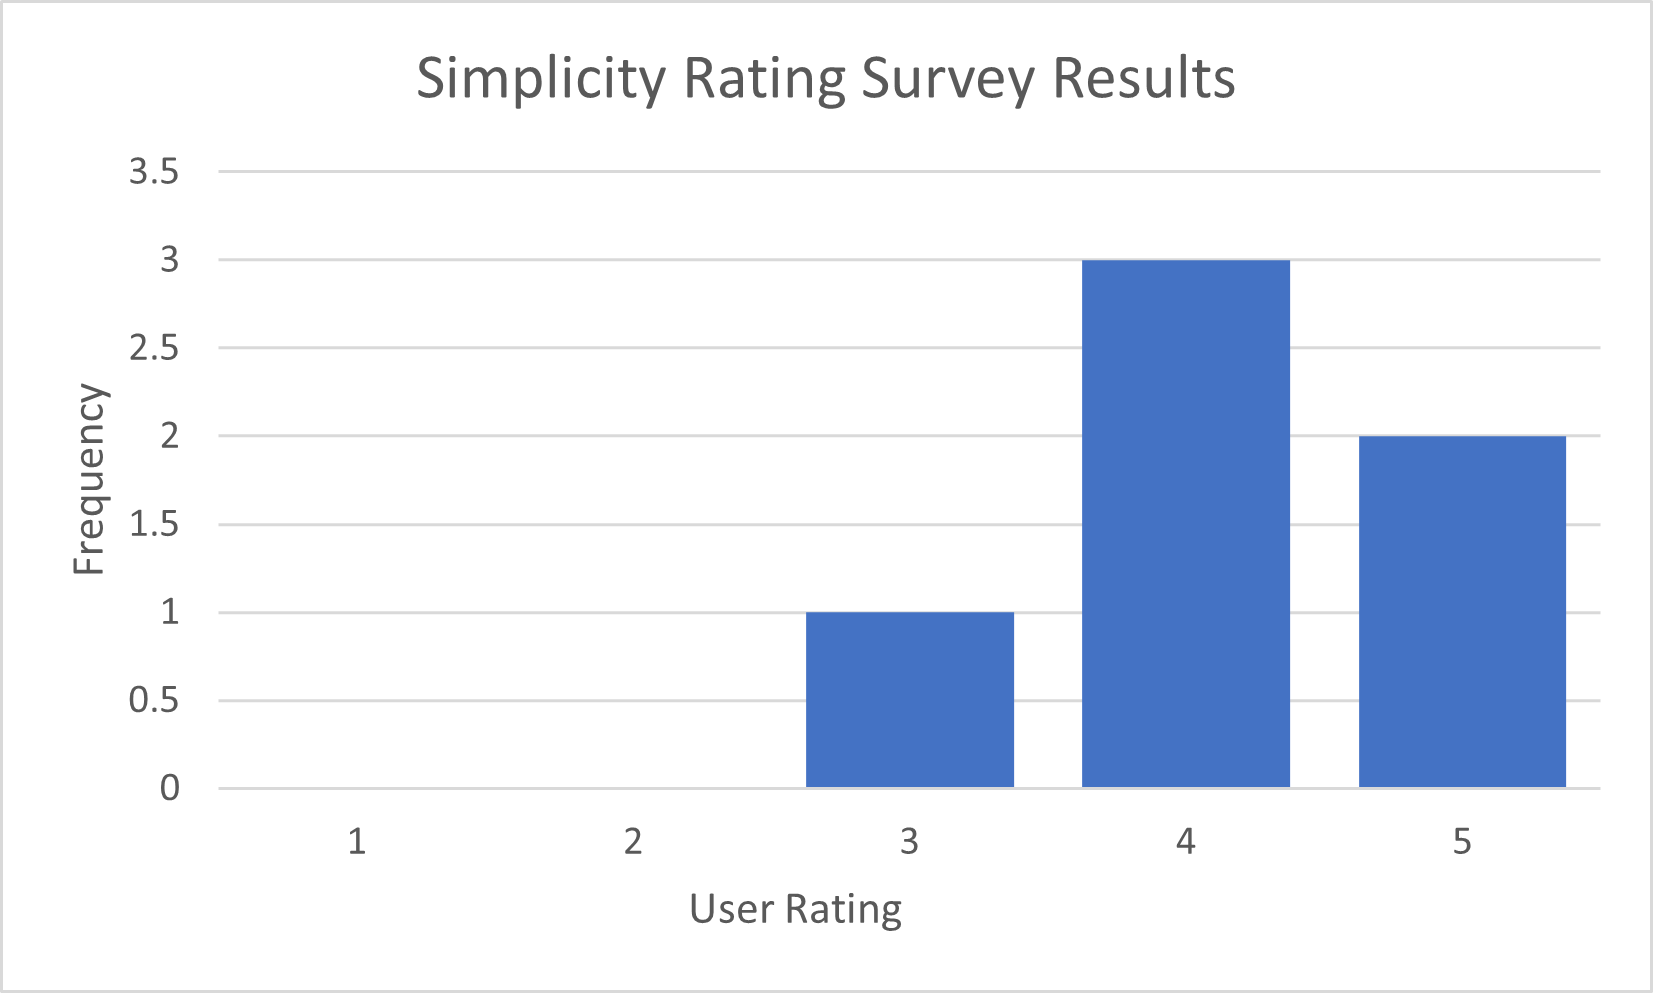
\includegraphics[]{simplicitysurvey}
\caption{Simplicity Survey}
\end{figure}

\subsubsection{Learning Time Observation ST-53}
Observation were done to record the learning time of first time users using the application. All the collected learning time were below the fit criterion threshold that was set initially \textcolor{green}{PASS}
\begin{figure}[H]
\centering
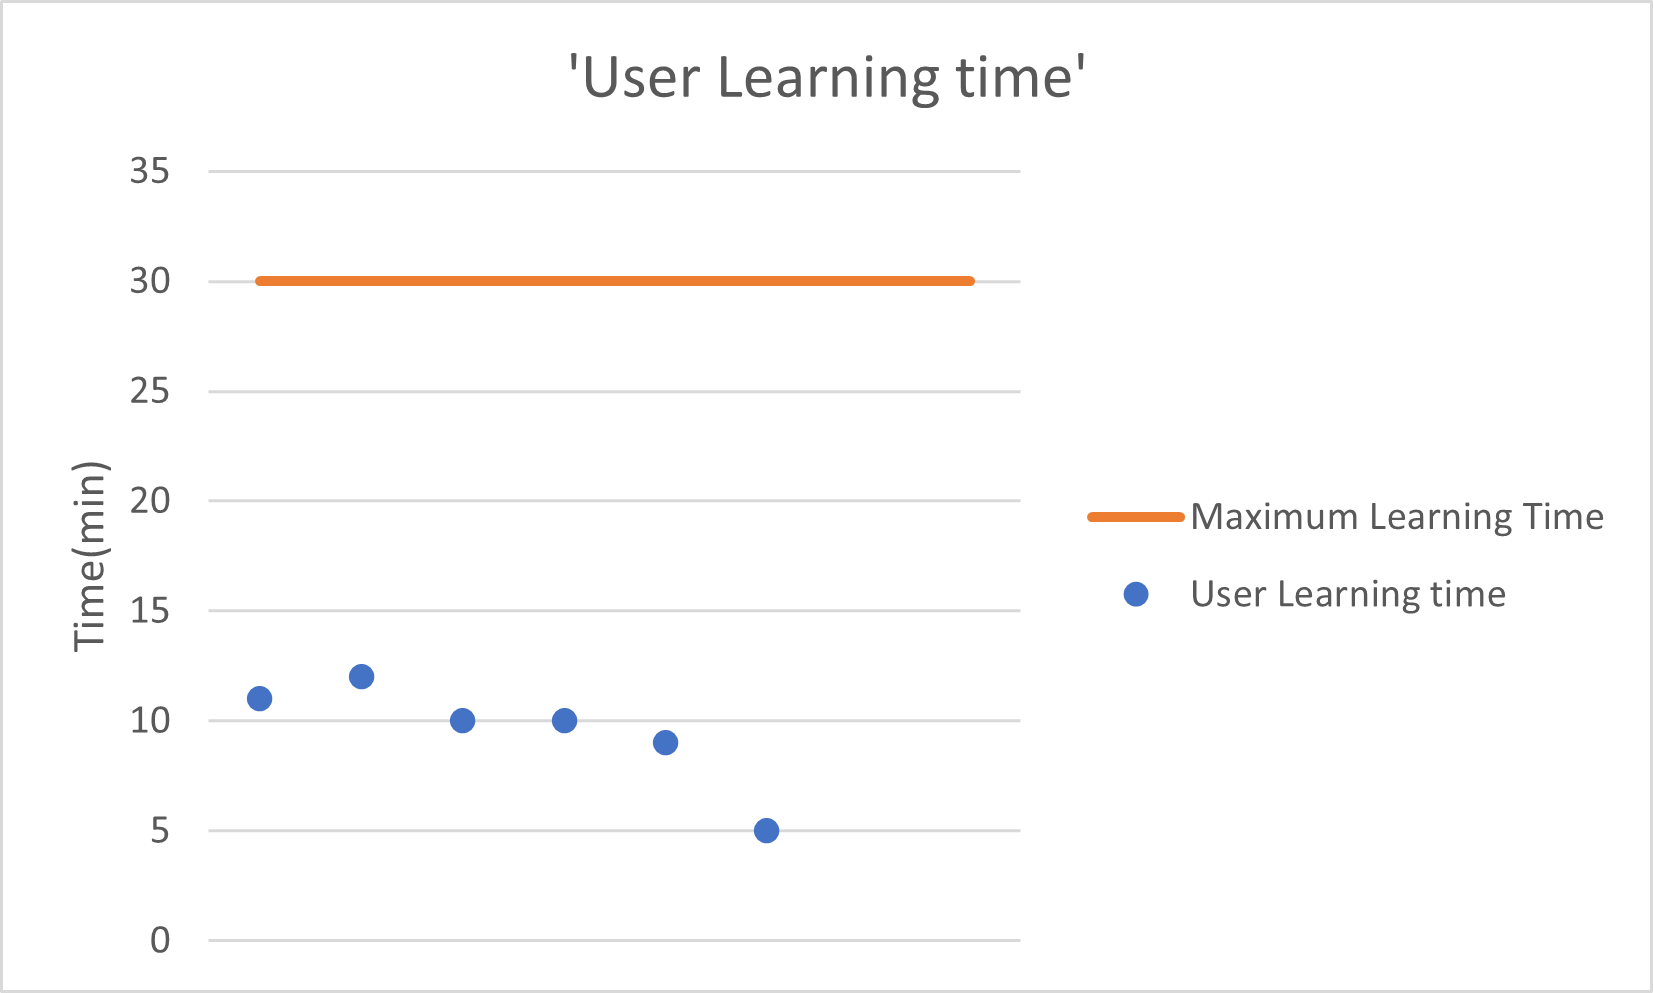
\includegraphics[]{learningtime}
\caption{Learnign Time Survey Result}
\end{figure}

\subsubsection{Easiness Survey ST-53}
A survey was done to rate the easiness of the application between 1-5. All the collected simplicity rating were within our initial fit criterion threshold \textcolor{green}{PASS}
\begin{figure}[H]
\centering
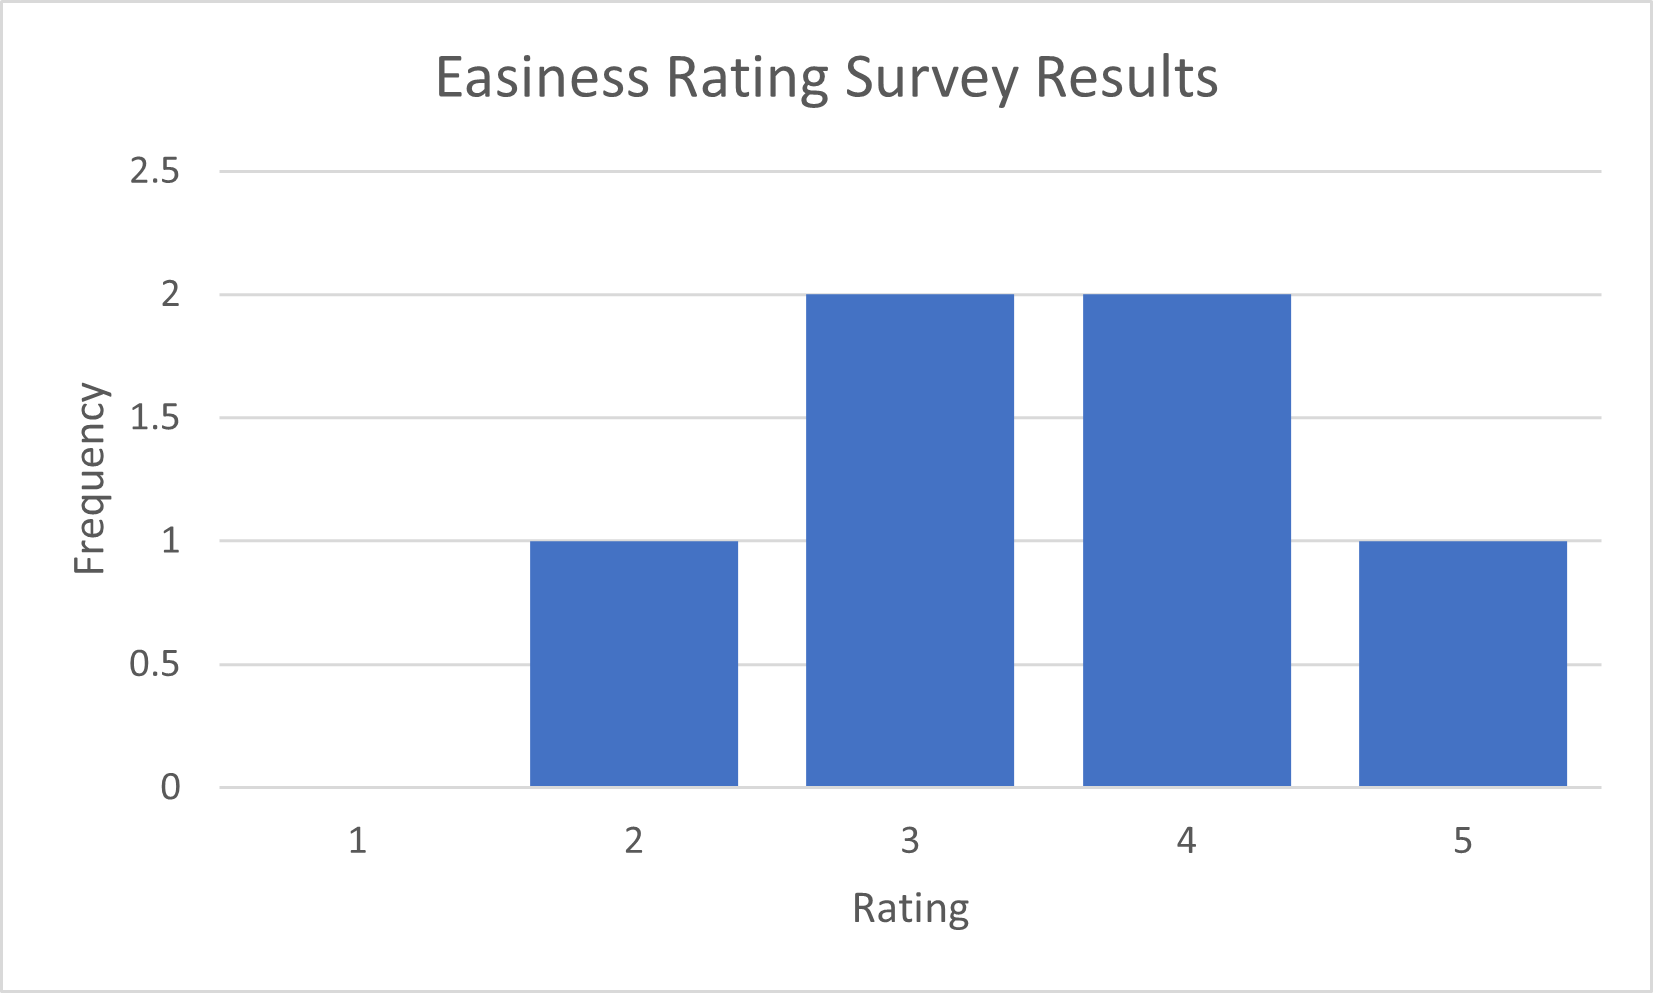
\includegraphics[]{easiness}
\caption{Easiness Survey Result}
\end{figure}

\subsubsection{Responsiveness Survey ST-55}
A survey was done to rate the responsiveness of the application between 1-5. All the collected simplicity rating were not within our initial fit criterion threshold \textcolor{red}{FAIL}
\begin{figure}[H]
\centering
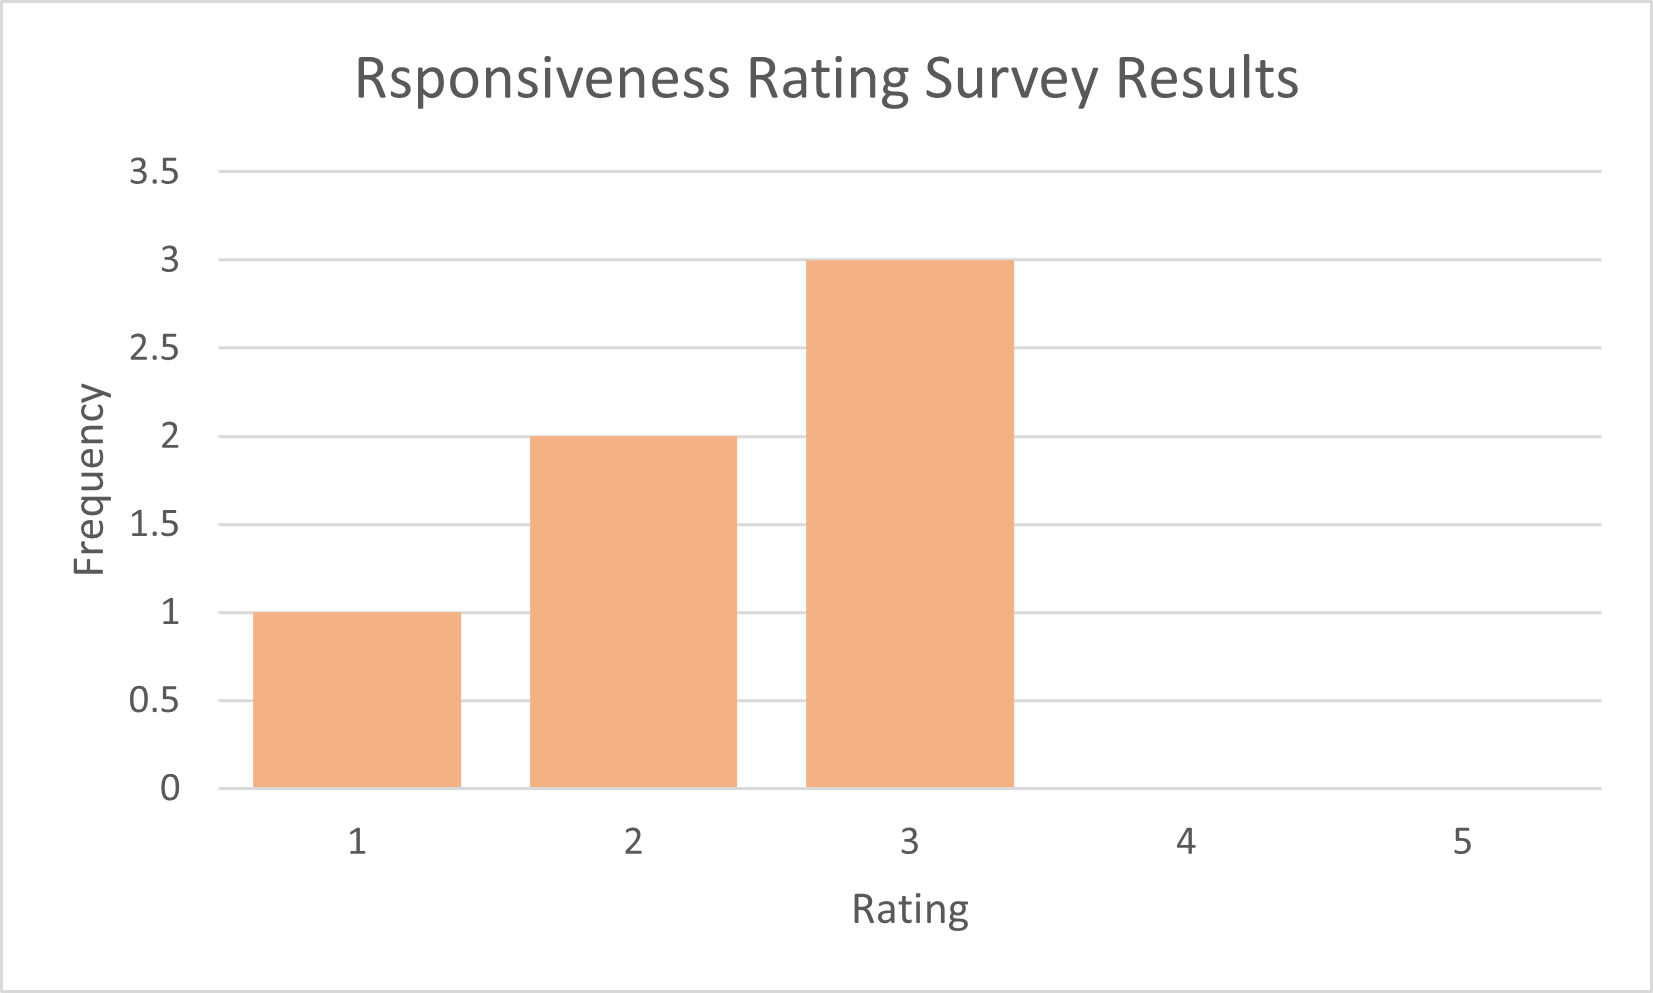
\includegraphics[]{responsiveness}
\caption{Responsive Survey Result}
\end{figure}


\newpage
\subsection{Other NFR tests}

\begin{center}
    \begin{longtable}{|c|p{1.2cm}|p{2.7cm}|p{3cm}|p{3cm}|c|}
        \caption{Project Services Unit Tests \label{long}}\\
        \hline
        \textbf{Id} & \textbf{Req Id} & \textbf{Input} & \textbf{Expected Result} & \textbf{Actual Result} & \textbf{Result}   \\
        \hline
        ST-51 & NFR2  & Tester checks the different number of colours used throughout the application excluding the syntax highlighting in the editor & No more than $\hyperlink{num_colours}{NUM\_COL}$ are different that main colour & No more than $\hyperlink{num_colours}{NUM\_COL}$ are different that main colour &  \textcolor{green}{PASS} \\
        \hline
        ST-52 & NFR3 & Tester confirms different user's cursors have distinct colours & Different user's cursors have distinct colours & Different user's cursors have distinct colours &  \textcolor{green}{PASS} \\
        \hline
        ST-56 & NFR11 & Tester checks the amount of time it takes to for the compiled PDF to appear from the time the button is pressed & The time taken is less than than $\hyperlink{compile_time}{COMP\_TIME}$ seconds & The time taken is more than $\hyperlink{compile_time}{COMP\_TIME}$ seconds &  \textcolor{red}{FAIL} \\
        \hline
        ST-59 & NFR16 & Developers on the team are surveyed on the maintainability of the application using a 1-5 rating & The average rating is greater or equal to $\hyperlink{maintain}{M\_RATING}$ seconds & The average rating is greater or equal to $\hyperlink{maintain}{M\_RATING}$ seconds &  \textcolor{green}{PASS} \\
        \hline
        ST-61 & NFR20 & Developers will check the project roadmap & Roadmap should indicate project will be done by deadline & Roadmap indicates project will be done by deadline &  \textcolor{yellow}{TBD} \\
        \hline
        ST-62 & NFR21 NFR22 & N/A & The system is fully documented & The system is fully documented &  \textcolor{green}{{PASS}} \\
        \hline
        ST-63 & NFR23 & Tester runs the application and does common tasks on chromium based browser, Firefox and Safari & The functionality of the application should be consistent across all these browsers & The functionality of the application should be consistent across all these browsers &  \textcolor{green}{PASS} \\
        \hline
        ST-65 & NFR26 & Tester will try to go to a project url that they do not have access to & The project URL should fail due to authorization error & The project URL fails due to authorization error &  \textcolor{green}{PASS} \\
        \hline
        ST-67 & NFR28 & Tester will note all system issues that happen in the application & All errors should have a message provided to the user & All errors have a message provided to the use &  \textcolor{green}{PASS} \\
        \hline
        ST-68 & NFR29 & Tester will try out all crucial actions in the application & All crucial actions should have a confirmation dialog & All crucial actions have a confirmation dialog &  \textcolor{green}{PASS} \\
        \hline
        ST-73 & NFR34 & Tester will disconnect from the internet and make some changes in the document currently being edited, and reconnect to internet & The changes to the editor should  get synchronized with other users & The changes to the editor get synchronized with other users &  \textcolor{green}{PASS} \\
        \hline
        ST-75 & NFR36 & Tester will try accessing projects page using URL without logging in & The project page should not be available & The project page is not be available &  \textcolor{green}{PASS} \\
        \hline
        ST-76 & NFR38 & Tester checks the values of the user credentials in the database & The user credentials should be encrypted & The user credentials are encrypted &  \textcolor{green}{PASS} \\
        \hline
        ST-77 & NFR39 & Tester checks the API keys in some hourly interval & The API keys should be different & The api keys are different &  \textcolor{green}{PASS} \\
        \hline
        ST-78 & NFR40 & Tester opens application and waits for browser session time out and then will access the projects page & The application should ask to re-authenticate & The application asks to re-authenticate &  \textcolor{green}{PASS} \\
        \hline
        ST-79 & NFR43 & Tester collects all the media on the application that is there by default  & All media on the application should be copy-right free & All media on the application are copy-right free &  \textcolor{green}{PASS} \\
        \hline
    \end{longtable}
\end{center}
	
\section{Comparison to Existing Implementation}	

N/A

\section{Unit Testing}

\subsection{Project Services Module}

\begin{center}
    \begin{longtable}{|c|p{1cm}|p{2.7cm}|p{3cm}|p{3cm}|c|}
        \caption{Project Services Unit Tests \label{long}}\\
        \hline
        \textbf{Id} & \textbf{Req Id} & \textbf{Input} & \textbf{Expected Result} & \textbf{Actual Result} & \textbf{Result}   \\
        \hline
        PS-1 & FR5  & User inputs a project name, and no collaborators and creates project & A project with the given name is saved in the database  &  A project with the given name is saved in the database &  \textcolor{green}{PASS} \\
        \hline
        PS-2 & FR5, FR6  & User inputs a project name, and a valid GitHub username as a collaborator & A project with the given name and collaborators is saved in the database & A project with the given name and collaborators is saved in the database &  \textcolor{green}{PASS} \\
        \hline
        PS-3 & FR5 & User inputs the name of the existing project to try and recreate it & The user gets an error that the project with the given name already exists & The user gets an error that the project with the given name already exists &  \textcolor{green}{PASS} \\
        \hline
        PS-4 & FR8, FR9, FR10  & User imports a project & A project with the correct name, collaborators, and files is added to the database & A project with the correct name, collaborators, and files is added to the database &  \textcolor{green}{PASS} \\
        \hline
        PS-5 & FR11, FR12  & User deletes a project & The project no longer exists in the database & The project no longer exists in the database &  \textcolor{green}{PASS} \\
        \hline
        PS-6 & FR11, FR12  & User deletes a project that does not exist & The user gets an error stating that the project does not exist & The user gets an error stating that the project has already been deleted &  \textcolor{green}{PASS} \\
        \hline
        PS-7 & FR13, FR14 & User asks to see all their projects & The user get both the project that they have created and the project that they are a collaborator of, but not the project that they are not a part of & The user get both the project that they have created and the project that they are a collaborator of, but not the project that they are not a part of &  \textcolor{green}{PASS} \\
        \hline
        PS-8 & FR16 & User adds a collaborator with a valid username to the project & The collaborator is added to the project in the database & The collaborator is added to the project in the database &  \textcolor{green}{PASS} \\
        \hline
        PS-9 & FR17 & User removes an existing collaborator from their project & The collaborator is removed from the project in the database & The collaborator is removed from the project in the database &  \textcolor{green}{PASS} \\
        \hline
    \end{longtable}
\end{center}

\subsection{File Services Module}

\begin{center}
    \begin{longtable}{|c|p{1cm}|p{2.7cm}|p{3cm}|p{3cm}|c|}
        \caption{File Services Unit Tests \label{long}}\\
        \hline
        \textbf{Id} & \textbf{Req Id} & \textbf{Input} & \textbf{Expected Result} & \textbf{Actual Result} & \textbf{Result}   \\
        \hline
        FS-1 & FR36, FR37 & User compiles an empty TeX file & The user should be given an error that the TeX file is empty & The TeX file does not compile successfuly and gives an error &  \textcolor{green}{PASS} \\
        \hline
        FS-2 & FR36, FR38 & User compiles a valid TeX file & The user is given a success message for the latex file being successfully compiled & The user is given a success message for the latex file being successfully compiled &  \textcolor{green}{PASS} \\
        \hline
        FS-3 & FR39 & User wants to access the PDF for a file that is not compiled yet & The user gets an empty PDF file returned to them & The user gets an empty PDF file returned to them &  \textcolor{green}{PASS} \\
        \hline
        FS-4 & FR39 &  User wants to access the PDF for a file that is compiled already & The user gets a valid PDF for the compiled file & The user gets a valid PDF for the compiled file &  \textcolor{green}{PASS} \\
        \hline
    \end{longtable}
\end{center}

\subsection{Chat Services Module}

\begin{center}
    \begin{longtable}{|c|p{1cm}|p{2.7cm}|p{3cm}|p{3cm}|c|}
        \caption{Chat Services Unit Tests \label{long}}\\
        \hline
        \textbf{Id} & \textbf{Req Id} & \textbf{Input} & \textbf{Expected Result} & \textbf{Actual Result} & \textbf{Result}   \\
        \hline
        CS-1 & FR42, FR43, FR44 & One user types a message and presses Send & The message content and metadata (sender, timestamp, UUID) are stored in the database & An entry for the message and metadata is created in the table  &  \textcolor{green}{PASS} \\
        \hline
        CS-2 & FR42, FR43, FR44 & One user types a message and presses Send & The user's Github profile picture is displayed next to their message & The user's Github profile picture is displayed &  \textcolor{green}{PASS} \\
        \hline
        CS-3 & FR42, FR43, FR44 & One user types a message and presses Send &  The message is displayed in the chat-box & The message is displayed in the chat-box &  \textcolor{green}{PASS} \\
        \hline
    \end{longtable}
\end{center}

\subsection{Auth Services Module}

\begin{center}
    \begin{longtable}{|c|p{1cm}|p{2.7cm}|p{3cm}|p{3cm}|c|}
        \caption{Auth Services Unit Tests \label{long}}\\
        \hline
        \textbf{Id} & \textbf{Req Id} & \textbf{Input} & \textbf{Expected Result} & \textbf{Actual Result} & \textbf{Result}   \\
        \hline
        AS-1 & FR3 & User clicks the Get Started or Login button, and then is redirected to the GitHub login page to enter credentials to be validated & User is able to view the projects home page in UnderTree once logged in, and their user data is saved into the database & User is redirected back to the UnderTree projects page and their user data is stored in the database &  \textcolor{green}{PASS} \\
        \hline
        AS-2 & FR4 & User is not authenticated and then tries to enter a restricted route in UnderTree & User is denied access since the user is not logged in, in the database, so the user is redirected to the login page to gain authentication & User is not able to access the restricted route and has to log in & \textcolor{green}{PASS} \\
        \hline
        AS-3 & FR4 & User is authenticated and then clicks log out & User is redirected back to the UnderTree home page access and the user isn't authenticated in the database & User is taken to the homepage and the database reflects their lack of authentication & \textcolor{green}{PASS} \\
        \hline
    \end{longtable}
\end{center}
\section{Changes Due to Testing}

%\wss{This section should highlight how feedback from the users and from 
% the supervisor (when one exists) shaped the final product.  In particular 
% the feedback from the Rev 0 demo to the supervisor (or to potential users) 
% should be highlighted.}

Throughout the development of this project, testing played a big part helping clarify and modifying the functionalities and the completeness of the services. After testing and validation we were able to confirm that the following changes would be needed to finalize this project:

\begin{enumerate}
    \item Add spell checking since this is a missing functionality\
    \item Delete, and modify functionalities are not fully complete since removing or renaming a file does not update the change for other users until they refresh
    \item Using user feedback we were able to tell that having to enter in a path name when creating or renaming a file increases the complexity of the user interface
    \item Having access to additional file types such as .bib files and potentially code files to be able to import code snippets into LaTeX may be helpful
    \item The functionality to commit files and add commit messages is not fully done since deleted files are not updated in the repository
    \item Accessing large TeX files from the editor is slow and negatively impacts the user experience which was reflected in our responsiveness survey. Thus, changes are currently being made to load documents when project loads, rather than when file is opened
    \item A big issue most users had during our usability testing was them forgetting to select the checkbox before pressing upload, thus that functionality has been tweaked such the commit button is visibly disabled until files are selected
\end{enumerate}

\section{Automated Testing}

All unit tests that are described above are done using automated testing using the Jest testing framework. This is a extremely useful framework since it allows us to easily mock any of the more complex features such as the GitHub integration which is out of scope as it would require integration testing rather than unit testing to be fully tested. Having these unit tests run after making a new change helps us be confident that all features are still functioning as intended. Additionally adding the unit tests into our CI/CD pipeline helps us ensure that any new commits to the main branch do not break the functionality of the project.

\newpage

\section{Trace to Requirements}

System Test Traceability can be accessed in the \href{https://github.com/RutheniumVI/UnderTree/blob/main/docs/VnVPlan/VnVPlan.pdf}{VNV Plan}

\begin{longtable}{|l|l|}
    \caption{Traceability Matrix between FR \& Unit Test Cases}\\
    \hline
    Functional Requirement &  Test Case\\
    \hline
    FR3  & AS-1 \\
    FR4  & AS-2, AS-3 \\
    FR5  & PS-1, PS-2, PS-3\\
    FR6  & PS-2\\
    FR8  & PS-4\\
    FR9  & PS-4\\
    FR10  & PS-4\\
    FR11  & PS-5, PS-6\\
    FR12  & PS-5, PS-6\\
    FR13  & PS-7\\
    FR14  & PS-7\\
    FR16  & PS-8 \\
    FR17  & PS-9\\
    FR36  & FS-1, FS-2\\
    FR37  & FS-1\\
    FR38  & FS-2\\
    FR39  & FS-3, FS-4\\
    FR42  & CS-1, CS-2, CS-3\\
    FR43  & CS-1, CS-2, CS-3\\
    FR44  & CS-1, CS-2, CS-3\\
    \hline
\end{longtable}
	
\section{Trace to Modules}

Traceability between modules and requirements can be accessed in the \href{https://github.com/RutheniumVI/UnderTree/blob/main/docs/Design/MG/MG.pdf}{Module Guide}

\section{Code Coverage Metrics}

N/A

\newpage
\section{Symbolic Parameters}

The definition of the requirements will likely call for SYMBOLIC\_CONSTANTS.
Their values are defined in this section for easy maintenance.\\

\noindent $\hypertarget{easiness_rating}{EASINESS\_RATING}$ = 7/10 \\
$\hypertarget{responsiveness_rating}{RESPONSIVENESS\_RATING}$ = 7/10 \\
$\hypertarget{compile_time}{COMP\_TIME}$ = 60 \\
$\hypertarget{learning_time}{LEARNING\_TIME}$  = 30\\
$\hypertarget{simplicity_rating}{SIMPLICITY\_RATING}$ = 8/10\\
$\hypertarget{num_colours}{NUM\_COL}$ = 4\\
$\hypertarget{uptime}{UPTIME} = 99$\\
$\hypertarget{maintain}{M\_RATING} = 4$\\
	

\bibliographystyle{plainnat}
\bibliography{../../refs/References}

\newpage{}

\section{References}

The following documents may be helpful in helping understand this document better:\\

\href{https://jestjs.io/docs/getting-started}{Jest Documentation for Unit Testing}

\href{https://github.com/RutheniumVI/UnderTree/blob/main/docs/VnVPlan/VnVPlan.pdf}{VNV Plan}

\href{https://github.com/RutheniumVI/UnderTree/blob/main/docs/Design/MG/MG.pdf}{Module Guide}

\section*{Appendix --- Reflection}

The information in this section will be used to evaluate the team members on the
graduate attribute of Reflection.  Please answer the following question: \\

% \begin{enumerate}
  % \item 
  In what ways was the Verification and Validation (VnV) Plan different
  from the activities that were actually conducted for VnV?  If there were
  differences, what changes required the modification in the plan?  Why did
  these changes occur?  Would you be able to anticipate these changes in future
  projects?  If there weren't any differences, how was your team able to clearly
  predict a feasible amount of effort and the right tasks needed to build the
  evidence that demonstrates the required quality?  (It is expected that most
  teams will have had to deviate from their original VnV Plan.)
% \end{enumerate}

\begin{enumerate}
    \item Faiq: Our original VnV plan was relatively simple and we assumed we would be easily able to unit test the vast majority of our project relatively simply. However once we got to actually implementing the unit tests, we realized the complexity of specific functionalities such as testing the GitHub integration that were located throughout our various services. For example, for creating a project we would need collaborators that were added to the project from our system to also be added to GitHub, however to actually have them fully added on GitHub, the user would need to first accept the invitation sent to their email. Thus, there is no simple way to unit test this and it starts to delve into the scope of integration testing since we would need to add the functionality of accepting the invitation and then checking GitHub to see if the collaborator has finally been added. Though this is possible in theory, we did not originally plan for this when writing our VnV plan and as a result did not allocate enough time to be able to go so far out of scope for our testing. Additionally, our original VnV plan also had relatively weak testing for the user interface and general usability. As we developed the project further, these usability tests were modified to help us get better user feedback on how we could improve when doing the VnV report. The need for most of these changes came from our lack of understanding of JavaScript testing frameworks, and lack of attention paid to hidden features such as the required GitHub utilities in the various functionalities of the project. In the future, these changes could have been predicted by better paying attention to how each functionality could be tested while developing, or instead even following test driven development so these issues could have been caught earlier. Aside from these changes, our system tests did not have any issues. This is because we were heavily focusing on rigorously testing our project with the system tests as we were developing for the various demonstrations. With the heavy focused placed on testing of the core functionalities, we had enough evidence that our project demonstrates the required quality from the various system tests associated with both the functional and non functional requirements. From the various data we collected from the non functional tests it is evident that though, we require some changes which are outlined in the changes made due to testing section, these changes will be easy to implement to meet the required quality.
    \item Veerash: After finishing this report, I have realized a lot has changed since the original design, but that is the reason we need to fake the design process. One main way our report is different than the plan is through the NFR. A lot of the ways the NFR were originally planned to be tested were not feasible testing methods. The reason for this was that some of our NFRs were not verifiable in the first place and they should have been reworded or removed. To fix this in the reports, some of these NFRs were removed. This experience has taught me the lesson to come up with verifiable NFRs from the start rather than having to backtrack everything. After testing some off these NFRs, it also came to realization that some of criteria for success were unfeasible. This naturally happens in a lot of projects where we do not have the knowledge to correctly evaluate what is the threshold that is needed to consider a NFR successful. Thus these thresholds, for example, the expected rating in a survey had to be changed to accurately reflect our new knowledge that we gained about the software. These experience we gain will be greatly helpful in the future when we have to come up with ways to quantify our NFRs since we can base it of past knowledge. Another reason our report differed from our plan was the fact that when we were making the testing plans, we did not consider the functionality of these test cases under the lens of the tools we had such as Jest, the testing framework. Tests will needed to be written under the rules and constraints of the framework and these rules and constraints were not so obvious at the time the test plan was constructed since we have never used Jest before. Thus the way these tests had to be carried our had to vastly change, one such example is testing a api endpoint, but in our tests we did not have access to the authorization, thus the test had to be conducted directly on the lower level functions. The experience with a testing framework such as Jest will aid me in the future when I have to come with test plans since I will have the knowledge of the rules and the constraints of the tools being used.
    \item Kevin: There are several ways that we noticed were different from our initial VnV plan. The reason being that the software process is inherently complex and unpredictable, so there are unforeseen challenges or obstacles that may come up which would require us to pivot and change strategies or methods. One of the main differences is that certain features or requirements turned out to be harder to implement and test as we thought of before. Yes, I would anticipate these changes in the future by making sure that the VnV plan that I create would make sure it is flexible and adaptable to prepare for these changes. One way to implement this 

\end{enumerate}

\end{document}